\chapter{Architektur}\label{ch:method}

\section{Mikrosystemarchitektur}

Dieses Projekt lässt sich zunächst in mehrere kleinen Projekte unterteilen. 
Bei einem so großen Projekt lohnt es sich eine Mikroservice Architektur anzustreben, bei der jeder Teil für sich gesehen eine Aufgabe erfüllt und nicht auf der Zuverlässigkeit eines anderen Systems beruht. 
Diese Methode wird auch divide-and-conquer genannt. 

Um das Projekt weiter einzuordnen, bietet es sich an, vorab Anforderungen an das System zu stellen. 
Da das gesamte Projekt als eine Reihe von Mikroservices umgesetzt werden soll, werden folgend für jeden Mikroservice Einzelne Anforderungen gestellt: 

\section{Anforderungen}

Zunächst muss die Datengrundlage geschafft werden. 
Dafür müssen die Podcast Epsioden heruntergeladen, transkribiert und anschließend alle Sätze in der Datenbank abgespeichert werden.
Dieses System muss in der Lage dem Titel eines Podcasts bzw. der ID in der Audiothek, sämtliche noch nicht in der Datenbank gespeicherten Episoden herunterzuladen, zu transkribieren und abzuspeichern.
In der Zukunft könnte man darüber nachdenken, diesen Teil komplett auf der Serverseite der ARD Audiothek laufen zu lassen.

Das nächste Mikrosystem muss in der Lage sein, diese Transkriptdaten in eine Form umzuwandeln, in der eine Suchfunktion relevante Abschnitte aus diesen Daten extrahieren kann.
Dafür soll es die einzelnen Wörter in sinnvolle Abschnitte Gruppieren und ein Embedding für jeden Abschnitt berechnen.

Ein weiterer Service soll dann die Suchfunktion übernehmen, indem er Stichworte oder Sätze als Parameter erhält und zu diesen die eine bestimmte Anszahl an relevanten Abschnitten zurückgibt.

Diese relevanten Abschnitte können noch weiter von ChatGPT analysiert werden, um zum Besipiel eine Auswahl aus vielen Dokumenten zu treffen, die Reihenfolge der Abschnitte zu bestimmen, oder ähnliche Themen herauszufinden.

Der nächste Service muss in der Lage sein, eine Liste an Segmenten entgegenzunehmen und daraus eine Audiodatei zu erzeugen.
Dafür muss er die originaldatein an den richtigen Stellen schneiden und die Audioschnipsel zusammenfügen können.

Als letztes muss die Audiodatei ausgeliefert werden. 
Dafür soll einmal eine API implementiert werden.
Außerdem soll ein UI als Webseite aufgbaut werden, welche die Anfrage in einem Formular entgegennimmt und dann die Audiodatei ausliefert.


\section{Vorgehensweise}


Zunächst müssen die Daten gesammelt und aufbereitet werden. 
Für dieses Projekt bildet die Datengrundlage die Transkripte, bzw. Manuskripte der Podcasts der ARD-Audiothek. 
In der Audiothek selber gibt es keine Transkripte zu den Podcasts. 
Für den Podcast „radiowissen“ von bayern2 gibt es auf deren Seite die Manuskripte in PDF Format. 
Diese sind zwar inhaltlich hochqualitativ, da Sie exakte Wortwahl der Podcasts enthalten, als PDF Format sind sie allerdings schwierig maschinell auszulesen und weiterhin besitzen sie keine Zeitinformationen zu den einzelnen Wörtern. 
Die Zeitinformationen in Form von Zeitstempeln für jedes Wort sind wichtig, um die Audiofiles der Podcasts später an den richtigen Stellen zuzuschneiden. 

Ein anderer Ansatz ergibt sich, wenn man die Podcasts transkribiert. 
Die Vorteile sind, dass die Transkription auch bei Podcasts funktioniert, für die vorab kein Transkript erstellt wurde, was die Mehrzahl aller Podcasts ausmacht. 
Außerdem kann man bei einer Transkription auch gleichzeitig die Zeitstempel für jedes Wort extrahieren.

\section{Programmiersprache Python}

In dieser Arbeit wird die Programmiersprache Python verwendet.
Python zählt zu den am meißten verwendeten Programmiersprachen weltweit und ist laut dem TIOBE-Index im Jahr 2023 sogar die meißt verwendete Programmiersprache überhaupt \cite{index2023}.
In dieser Arbeit wird Python verwendet, da es Unterstützung für sehr gute Bibliotheken für Machine Learning und NLP Anwendungen gibt.
Vor allem die Unterstützung für Transformermodelle mit der Bibliothek transformers, die NLP Bibliothek SpaCy, sowie Datenverwaltungsbibliotheken wie pandas und support für SQLite Datenbanken mit sqlite sind sehr praktisch.
Dazu ist Python sehr einfach zu verstehen und rechenaufwändige Operationen wie in der transformers Bibliothek sind sehr performant in der Sprache C implementiert.



\section{Transkription der Podcasts}


\subsection{Fraunhofer}

Seit 2015 arbeitet die ARD mit dem Fraunhofer-Institut Institut für Intelligente Analyse- und Informationssysteme (IAIS) zusammen, um „Erschließung von Mediendaten zu forcieren und dabei den Schwerpunkt auf maschinelle Verfahren zu legen“ [1]
Ein Teil dieses Projektes bezieht sich auf das Audio-Mining. 
Das Fraunhofer IAIS entwickelte dafür ein System, welches die Audiodatein transkribiert und dabei „in der kompletten ARD, bei Deutschlandradio sowie im ZDF im Einsatz [ist]“. 
Leider legt das FraunhoferIAIS nicht offen, welche Technologie es dafür verwendet. 
Die Transkripte lassen sich allerdings sehr einfach über eine Graphql Schnittstelle abfragen. 

\subsection{Microsoft Translate}

Eine weitere Möglichkeit zur Audiotranskription bietet Microsoft Translate. 
Soweit man einen Microsoft 365 Account besitzt kann man in dem Webinterface von Microsoft word eine Transkriptionsfunktion benutzen. 
Dafür müssen die Audiofiles zunächst auf Microsoft Onedrive hochgeladen werden und können dann mit einem Klick übersetzt werden. 
Microsoft Word stellt dann sogar Timestamps  zur Verfügung für das ganze Dokument. 
Die Qualität ist außerdem besser als bei kostenlosen Open-Source Alternativen. 
Dafür skaliert diese Art der Transkription schlecht für größere Datenmengen, da sämtliche files zunächst bei OneDrive hochgeladen werden müssen und dann jedes File von Hand ausgewählt, in Word eingebunden, transkribiert werden und dann abgespeichert werden müssen. 

\subsection{Whisper}

Für die Transkription eignen sich Automatic Speech Recognition Systeme (ASR). 
Eines der besten kostenlosen ASR Systeme bietet Whisper von OpenAI. 
Dieses System wurde mit einem maschinellen lernverfahren auf 680 000 Stunden Audiomaterial in verschiedenen Sprachen trainiert. 
Es ist sehr leistungsstark und kann lokal auf eigener Hardware laufen. [2] [3]

Whisper bietet mehrere verschiedene Modelle zur Transkription an. Es gibt die Modelle tiny, base, small, medium und large. 
Das Basismodell hat ca. 74 Millionen Parameter und benötigt ca. 1 GB VRAM und ist ca. 16 mal schneller als das large Model. 
Bei einem Test für die Episode 1968-das-ausnahmejahr aus dem Podcast Radiowissen von br2 schneidet es aber nicht sehr gut ab. 
Aus dem Wort „Vietnam“ wird „Wirdnam“, aus „Panzer in Prag“ wird „Panzer-Inprac“ und aus  „Ohrfeige“ wird „Urfeige“. 
Der vorgetragene Text wurde dabei ohne Störgeräusche und von einer Person flüssig vorgetragen. 

Dagegen bietet das Medium Model von Whisper deutlich bessere Ergebnisse für die selbe Episode. 
Bei der Transkription konnte kein Fehler festgestellt werden. Allerdings ist der Zeitaufwand durch höhere Rechenleistung immens. 
Auf einem Macbook Pro 2016 mit einem Intel Core i7 benötigt die Transkription ca. 45 min. pro Episode. 
Auf einer T4 GPU, wie sie Google kostenlos auf Google Colab zur verfügung stellt, dauert eine Transkription immer noch 3,5 Minuten. 
Für ca. 1000 Episoden bräuchte man demnach ca. 3500 Minuten, d.h. ca. 58 h. 

Drawbacks von Whisper:
Medium Modell immer noch einige Fehler: 
- gubt statt Grub
- wenn Sprecherwechsel manchmal ganze Sätze weg (im-bann-des-mondes-archaische-mythen-und-religionen.mp3	)

TODO large ausprobieren, auf den Servern der Uni und mit der Ebu API
Eurovox


Die Transkripte der Episoden sind meißt ca. 3000 Wörter lang und benötigen ungefähr 20 KB Speicherplatz pro Transkript.

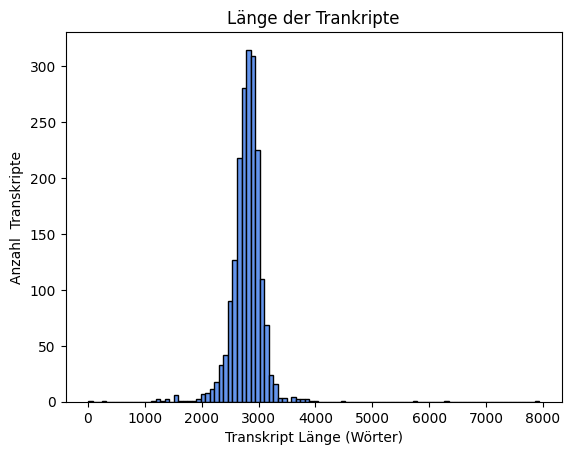
\includegraphics[width=\linewidth]{figures/transcript_length.png}


\subsection{Eurovox}

Das Problem der langen Wartezeiten lässt sich umgehen, wenn wir Cloud computing benutzen, das heißt, das Whisper model nicht auf der lokalen Hardware laufen zu lassen, sondern zum Beispiel auf den Servern von Eurovox. 
Eurovox ist ein Software tool von der EBU, der Europian Broadcast Union. 
Sie ist ein zusammenschluss von derzeit 68 Rundfunkanstalten in 56 Staaten Europas, Nordafrikas und Vorderasien mit Sitz in Genf. [4] 
Das tool Eurovox steht dabei allen Mitgliedern zur Verfügung.  
Mithilfe dieses Tools kann man Text-to-Speech, Übersetzungen und Speech-to-Text Services über eine UI benutzen. 
Es gibt sogar die Möglichkeit wärend eines Streams live audio captions zu erzeugen. 
Für dieses Projekt benutzen wir aber zunächst nur die Translation Funktion. 
Außerdem verwenden wir die API von Eurovox um später das ganze Projekt auf mehr Episode Transkripte ausweiten zu können. 
Laut den Entwicklern soll die API auch demnächst open-sourced werden [QUELLE].

Die API stellt, ebenso wie das Tool, eine Reihe verschiedener Anbieter zur verfügung, über die wir die Audios transkribieren lassen können. 


\section{Datenvorbereitung}

\subsection{Satzbildung}

Die transkribierten Daten, welche Whisper erzeugt enthalten die erkannten Wörter, sowie die einzelnen Zeitstempel für den Start und das Ende jedes Wortes mit einer genauigkeit von Zehntelsekunden.
Für die spätere Analyse der Daten, ist es Sinnvoll die einzelnen Wörter in größere Segmente zusammenzufassen, damit bei einer Suchfunktion der Kontext von erschiedenen Wörtern miteinbezogen werden kann.
Ein naheliegender Ansatz besteht darin, die einzelnen Wörter zunächst in Sätze zu gruppieren.
Für diese Gruppierung werden zwei Ansätze betrachtet.
Der einfachste Ansatz besteht darin, die von Whisper erzeugten Satzpunkte als  Trennzeichen für einen Satz zu zählen.
Whisper erkennt von sich aus aufgrund der Tonlage und der Pause zwischen Wörtern und der grammatikalischen Struktur der vorangegangenen Wörtern, ob ein Wort das Ende eines Satzes markiert. ???
Dann gibt Whisper das Wort mit einem Punkt, einem Fragezeichen, oder einem Ausrufezeichen am Ende als erkanntes Wort aus.
Diese Punktuation kann man benutzen, um die einzeln Wörter in Sätze zu gruppieren.
Leider ergibt sich dabei das Problem, dass bestimmte Wörter, oder Abkürzungen zusätzöiche Punkte enthalten.
Beispiele sind "Mr. Smith", "seinem 26. Studioalbum", "am 10. Januar 2016".
Mit diesem naiven Ansatz der Satztrennung, würden wir also einige Sätze an ungewollten Stellen in mehrere Sätze auftrennen.

Um dieses Problem zu lösen, muss der Algorithmus verstehen, welche Satzzeichen die wirklichen Satzenden sind.
Dies erfordert ein verständnis der Satzstruktur und ist deswegen nicht trivial möglich.
Um die Sätzegrenzen zu finden, wird deshalb die Open-Source Sprachbibliothek SpaCy.\cite{honnibal2017}

David Bowie stirbt am 10. Januar 2016 an Leberkrebs.
Zwei Tage nach seinem 69. Geburtstag und der Veröffentlichung von Blackstar, seinem 26. Studioalbum.

\subsection{Satzbildung mit SpaCy}

Mithilfe der NLP Bibliothek SpaCy kann man herausfinden, welche Satzzeichen wirklich die Grenze eines Satzes Markieren.
SpaCy verwendet dafür Machine Learning Modelle, die aufgrund von vielen Daten gelernt haben, wo das Ende eines Satzes ist.
Es gibt auch noch die beliebte Bibliothek NLKT, die sich aber eher auf das Unterrichten von NLP spezialisiert hat.
SpaCy ist eher für den produktiven Einsatz geeignet.
Auf der offiziellen Webseite von spaCy werden vier verschiedene Modelle für die deutsche Sprache zur verfügung gestellt.
Das Modell 
\begin{verbatim}
    de_core_news_sm 
\end{verbatim} 
ist das kleinste Modell mit 13 MB Größe, dann folgt 
\begin{verbatim} 
    de_core_news_md 
\end{verbatim}
mit einer Größe von 42 MB und 
\begin{verbatim}
    de_core_news_lg 
\end{verbatim}
ist das größte Modell mit 541 MB.
Das größte Modell bietet dabei vor allem viele vortrainierte Embedding Vektoren für einzelne Wörter.
Das vierte Modell ist 
\begin{verbatim}
    de_dep_news_trf
\end{verbatim}
verbraucht 391 MB Speicherplatz und ist speziell für Transformer-support geeignet.
spaCy führt eine selbst angegebenen Accuracy Evaluation für Sentence Segmentation, also das Erkennen von Satzenden in einem Text.
Darin ist der F-Score für das kleine Modell gleich 0,94; für das mittlere Modell 0,95 und für das große Modell ebenfalls 0,95.
Das Modell mit der Transformer pipeline bietet einen F-score von 0,98 und wird deswegen in dieser Arbeit verwendet. \cite{spacy2024}


\subsection{Sätze Normalisieren / cleanen}

Für Retrieval funktionen ist es Sinnvoll, mehrere Wörter zusammenzufassen.
Wenn man einen Algorithmus hat, der gezielt Wörter im Korpus suchen kann, ist es Wünschenswert nicht nur exakt die selben Wörter zu suchen, sondern auch verwandte Wörter.
Zum Beispiel sollte die Suche nach dem Wort "Wanderer" auch Ergebisse für die Worte "Wandererin", "Wanderung" oder "wandern" enthalten, nicht aber das Wort "Wand".

\subsubsection{Tokenisierer}

In Machine Leerning Anwendungen nutzt man dafür verschiedene Tokenisierer.
Es gibt einfache Tokenisierer, wie Whitespace Tokenisierer, die einen Text einfach an Leerzeichen teilen und die einzelnen Wörter als Tokens behandeln.
Etwas besser sind Wort Tokenizer, die auch Satzzeichen erkennen und dadurch Punkte und Kommata nicht an das Ende des vorangegangenen Wortes anhängen. 
Einen solchen Tokenizer nutzt beispielsweise spaCy, um "Linguistic Features" zu bestimmen.
Es gibt Subword tokenisierer, die Worte nocheinmal in kleinere Abschnitte teilen.
Das Byte-Pair Encoding versucht aufgrund von Statistischen Methoden, häufig vorkommende zusammenhängende Zeichenfolgen als Tokens zu identifizieren.
Diese Art Tokenizer wird zum Beispiel oft für die Eingabe bei Transformern genutzt. [Quelle]
Die Transformermodelle von OpenAI benutzen beispielsweise tiktoken als Tokenizer [Quelle], das BERT Modell von Google benutzt den WordPiece Tokenizer.



\subsubsection{Lemmatisierung vs. Stemming}

Um diese Abbildung von mehreren Worten auf ein Stammwort zu erreichen, gibt es zwei unterschiedliche Methoden:
Die Methode Stemming versucht regelbasiert Suffixe von Worten zu ersetzen, um aus Wörtern mit verschiedenen Endungen, wie zum Beispiel "Wanderer" und "Wanderung" zu einem Wort "Wander" zu reduzieren.
Der Vorteil ist, dass der Algorithmus sehr schnell agieren kann, um die Worte auf ihre Stammform zu reduzieren.
Die Nachteile sind allerdings, dass die Deutsche Sprache sehr viele verschiedene Wortkonstrukte erlaubt, die nicht alle mithilfe von einzelnen Regeln auf ein gemeinsammes Stammwort gebracht werden können. 
Zum Beispiel bei dem Plural von "Baum"; "Bäume".


\subsubsection{Kompositatrennung Pyphen vs german compound splitter}

Als weiteren Vorverarbeitungsschritt für die effiziente Keywordsuche kann man zusammengesetzte Wörter in ihre bestandteile auftrennen.
Das Vokabular des Datensazes besteht zu 61\% aus Nomen. 
Die meisten der Nomen sind zusammengesetzte Nomen, manche davon sind sehr lang, wie zum Beispiel "reichsdeputationshauptschlussakte", oder "hochgeschwindigkeitstransportmittel".
In dem ganzen Vokabular, das aus den Transkriptionen von Whisper stammt, besteht fast die Hälfte (47,8\%) aus zehn oder mehr Buchstaben.
Da für exakte Keywortsuche solche Begriffe fast nie auftreten, lohnt es sich, 

\section{Transktript Segment Ranking}

\subsection{Ählichkeitssuche lexikalisch}

\subsubsection{Keywordsuche}

Eine Möglichkeit bietet sich in der Keywordsuche. 
Hierbei wird einfach überprüft, ob sich ein Keyword in einem der Dokumente wiederfindet. Ist die möchte ein User beispielsweise einen zusammengeschnittene Podcast Episode über „Zugspitze“, so schaut das System, in welchen Episodensegmenten das Wort „Zugspitze“ auftaucht, und gibt diese zurück. 
Schwieriger wird es, wenn die Useranfrage mehrere Wörter beinhaltet. 
Möchte sich der User über das Thema „Zugspitze wandern“ informieren so müsste zunächst untersucht werden, welche Dokumente beide Worte enthalten, welche nur eines der beiden enthalten. 
Dann müsste man dementsprechend auch ein Algorithmus entwickeln, der diese dann sinnvoll hierarchisiert. 

\subsubsection{TF-IDF}

Einen solchen Ansatz bietet das TF-IDF Maß (Term Frequency – Inverse Document Frequency). 
Im Bereich des NLP verwendet man das TF-IDF Maß um zu untersuchen welche Wörter in verschiedenen Dokumenten welche Gewichtung erfahren. 
Dazu wird zunächst die TF-Matrix, also die Term Frequenzy Matrix berechnet. 
Hierbei wird erst das Vokabular ermittelt, also die Gesamtheit aller Tokens (Wörter) die es in allen Dokumenten (Transkript Segmenten) des Korpuses (alle heruntergeladenen Episoden) gibt. 
Dann wird für jedes einzelne Segment die Anzahl jeder in ihm auftretenden Tokens ermittelt. 
Für den Satz: „Auf der Zugspitze gibt es viele Wanderer, die die Zugspitze lieben“. 
In diesem Fall würde in der TF Matrix an der Stelle Zugspitze eine 2 Stehen, in der Zeile Wandern aber 0, da zwar das Wort Wanderer, aber nicht das Wort wandern vorkommt. 
Da diese beiden Worte aber sehr ähnlich sind und der User bei einer Anfrage nicht immer nach verschiedenen Versionen eines Wortes suchen will, um dann ein zufriedenstellendes Audio zu erhalten


Dabei gibt es allerdings keine Möglichkeit, die verschiedenen Treffer dieser suche nach Relevanz zu hierarchisieren. Sucht man zum Beispiel nach dem Stichwort „Klimakrise“ würden dabei mehrere Stunden Material zusammenkommen [QUELLE]. 
Man könnte nun einfach die Ersten Segmente nehmen, die zusammen die vorgegebene Zeit überbrücken. Allerdings ist dieser Ansatz wenig Vielversprechend. 


\subsection{Ähnlichkeitssuche Semantisch}

\subsubsection{Embeddings}

\subsection{Ähnlichkeitsvergleiche}

Mithilfe der Embedding Vektoren können können wir Sätze finden, die zueinander Ähnlich sind. Aber was bedeutet überhaupt ähnlich? Die Vektoren des BERT Models sind 768 Dimensional, haben also 768 Gleitkommazahlen gespeichert, die zwischen -1 und 1 liegen. 
Diese Gleitkommazahlen Vektoren könnte man auch als Feature Vektoren begreifen. 
Zum Beispiel könnte die erste Zahl dieses Vektors für die Erwähnung von Professoren in dem Satz stehen (-1 für keine Professoren; 1 für viele Professoren). 
Die zweite Zahl könnte für das Thema Essen stehen (-1 für wenig mit Essen zu tun; 1 für sehr viel mit Essen zu tun). 
Damit hätte der Satz „In der Mensa gibt es jeden Tag Currywurst mit Pommes“ an der ersten Stelle vielleicht eine 0,1, weil der Begriff „Mensa“ leicht mit Uni und Professoren konnotiert wird und die zweite Stelle würde bei 0,94 liegen, da es in dem Satz offensichtlich um das Essen handelt. 
In der Realität wird das Model sehr wahrscheinlich nicht so für Menschen offensichtlichen Merkmale lernen. Ein Grund dafür ist, dass das Model vor allem pro Eintrag eine linearkombination von verschiedenen Menschenoffensichtlichen Merkmalen lernen wird, also jede Zahl eine überlagerung verschiedener Eigenschaften darstellt. 
Eine forschungsrichtung, die versucht solche Modelausgaben Menschenlesbar zu gestalten liegt in der Explainable AI

Um die Ähnlichkeit von diesem Satz zu der Frage „“ zu bestimmen nutzen wir die Cosinus distanz als Maß. Es gibt auch die Euclidische Distanz, allerdings gestaltet sich dabei das Problem der Vector Normalisierung.


Diese Komplexen semantischen Unterschiede, oder Gemeinsamkeiten zu erkennen erfordert etwas mehr Raffinesse.

Andere Distanzmaßen:
Manhatten Distanz (nur x oder y Achse)
Hamming Distanz (Anzahl verschiedener Einträge)

\subsubsection{Euclidean Similarity}

Die Euklidische Distanz von zwei Vektoren kann man über den Satz des Pythagoras berechnen.
Dafür nimmt man für jede Dimension die Differenz beider Vektoren in dieser Dimension, quadriert diese und summiert alle Quadrate zusammen, um dann die quadratwurzel darüber zu ziehen.
Für die beiden Vektoren 
$\begin{pmatrix}0\\1\end{pmatrix}$
und 
$\begin{pmatrix}-1\\0\end{pmatrix}$
wäre die

Euklidische Distanz $\frac{1}{\sqrt{2}}$, da $\sqrt{(0-(-1))^2 + (1-0)^2}=\frac{1}{\sqrt{2}}$

Dieses Distanzmaß ist sensibel gegenüber der Länge der Vektoren.
Wenn die Vektoren nicht normiert wurden, kann die Euklidische Distanz sehr groß werden und die Ergebnisse einer Ähnlichkeitssuche verfälschen.


\subsubsection{Cosinus Similarity}

Ein weiteres Ähnlichkeitsmaß kann man über den Winkel zwischen zwei Vektoren definieren.
Dieser Winkel ist unanhängig davon, wie lang die Vektoren sind, immer gleich.
Die weitverbreiteste Methode um diesen Winkel zu messen, ist über die Cosinus Ähnlichkeit.
Diese berechnet den Cosinus des Winkels und kann einfach über die Formel

$\text{cosine\_similarity}(\mathbf{a}, \mathbf{b}) = \frac{\mathbf{a} \cdot \mathbf{b}}{\|\mathbf{a}\| \|\mathbf{b}\|}$

berechnet werden.
Dabei wird für beide Vektoren zunächst das Skalarprodukt bestimmt.
Das Skalarprodukt besitzt die Eigenschaft groß zu sein, wenn beide Vektoren in ähnliche Richtungen zeigen und kleiner, wenn beide Vektoren in unterschiedliche Richtungen zeigen.
Dabei hat die Länge der unterschiedlichen Vektoren einen Einfluss auf die Größe des Skalarproduktes.
Um dieser Verzerrung entgegenzuwirken, wird das Skalarprodukt durch das Produkt der Beträge der Vektoren geteilt.
Dadurch erhält man den cosinus des Winkels zwischen diesen beiden Vektoren.

Wenn beide Vektoren vorher normiert wurden, das heißt der Betrag der Vektoren gleich Eins ist, ist die Cosinus Distanz gleich der Skalarprodukt Distanz der beiden Vektoren.
Außerdem kann in diesem Fall die Euklidische Distanz asu der Cosinus Distanz errechnet werden durch die Formel: 

$\text{Euclidean distance} = \sqrt{2 - 2 \cos(\theta)}$

\subsection{Anreichern der Segmente}

Das Ranking der einzelnen Sätze liefert eine Auswahl der besten Kandidaten für den Podcast.
Einzelne Sätze, die aus verschiedenen Podcast Episoden stammen ohne Kontext hintereinander abzuspielen bietet für den Zuhörer nur ein mäßiges Hörerlebnis. 
Es fehlt der Kontext zu den einzelnen Informationen.
Zum Besipiel bekommt man für die Suchanfrage "Geschichte Amsterdam" mit dem TF-IDF Ansatz Sätze wie "Amsterdam, das bedeutet unbeschwerte Kinderjahre" oder "Amsterdam gefiel ihm".
Die Sätze an sich bieten kaum interessante Informationen.
Dem Zuhörer stellen sich sogar noch mehr Fragen, zum Beispiel für wen Amsterdam unbeschwerte Kinderjahre bedeuten oder wem Amsterdam gefiel.

Um dem Zuhörer mehr Informationen zu geben kann man die Größe der einzelnen Segmente Anpassen.
Dazu kann man mehrere Ansätze betrachten.
Der einfachste Ansatz ist, für jeden einzelnen Satz die umgebenden Sätze davor und dahinter miteinzubeziehen.
Die Anzahl der umgebenden Sätze ist dann ein Hyperparameter dieses Systems und kann vom Nutzer durch den Parameter Segmentlänge eingestellt werden, welher die Anzahl der Sätze in einem Segment angibt.
Falls der auszuschneidende Satz am Anfang oder am Ende des Transkriptes vorkommt, und die Segmentlänge so eingestellt ist, dass mehr Sätze als möglich dem Segment hinzugefügt werden sollten, so wird das Segment an der Transkriptgrenze abgeschnitten.
Die Evaluation der besten Segmentlänge wurde in dieser Arbeit nicht ausgeführt, als defaultwert ist für die Segmentlänge 5 eingestellt.

Ein weiterer Ansatz wäre auch hier ein mächtiges LLM, wie ChatGPT zu benutzen, um die richtige Segmentlänge für jedes Segment individuell einzustellen.
Dazu kann man das LLM instruieren, aus einer sehr großen Anzahl an Kontextsätzen (zum Beispiel 50) oder dem ganzen Transkript einer Podcast Episode und der dazugehörigen Frage, die Anzahl der Kontextsätze auf das wesentliche zu beschränken.

% Dieser Ansatz würde allerdings sehr zeit- und rechenaufwändig sein.
% Wenn man als LLM ChatGPT benutzen würde, dann würden pro einzelnem Segment ca. 50 Sätze (entspricht ca. 500 Tokens) ca. 0.00025 \$ kosten entstehen.

In dieser Arbeit wurde dieser Ansatz ausprobiert mithilfe eines Promptes wie 

Je nachdem welches LLM man dafür benutzt könnten Zeit und kostenfaktoren eine Rolle spielen.


\subsection{Ranking mit ChatGPT}

Nachdem nun die Einzelnen Sätze zu gößeren Segmenten erweitert wurden, kann man auch die Reihenfolge der einzelnen Segmente anpassen.
Wenn man sich beispielsweise über die "Geschichte von Amsterdam" informieren will, kommen dazu verschiedene Ausschnitte aus der Zeit der Gründung der Niederlande, der 



\section{Audio-Zusammensetzung}


Für die Bearbeitung von Audio files in Python bietet sich das Python Modul Pydub an. Mit diesem Modul kann man ein Audiofile ähnlich wie ein Array behandeln, aus dem man nun einen Abschnitt von Sekunde 2 bis Sekunde 4 schneiden möchte. 
Für die Zeitstempel der Start und End zeit jedes Audiosegments nehmen wir die Daten aus der sortierten Ranked segments.json Datei.
Diese werden dann als extra Audiofiles abgespeichert und im nächsten Schritt wieder Zusammengesetzt.

Um die Audios nun wieder zusammenzusetzen verwenden wir das gleiche Modul Pydub. Es bieten sich mehrere Möglichkeiten an, die Audiosegmente wieder zusammenzusetzen. Man könnte die Segmente einfach ohne Pause hintereinander abspielen. Dabei folgen allerdings mehrere Probleme: 
Zum einen werden die Audiofiles nicht immer an sehr passenden Stellen getrennt, sodass manchmal mitten im Wort abgebrochen wird und das nächste Segment beginnt. 
Um dieses Problem zu lösen könnte man die Audiofiles langsam ausfaden lassen.

Außerdem sollte dem Hörer bewusst sein, dass ein Audiosegment aus einer Episode aufhört und das nächste beginnt. 
Dafür bietet sich ein kurzer Signalton zwischen den einzelnen Audiosegmenten an. 
Dieser sollte nicht nervig sein, da er dem Hörer öfter vorgespielt wird. 

Eine weitere Möglichkeit wäre, zwischen jedem Segment dem Hörer eine kurze Vorstellung der Episode und der Sprecher*in zu ermöglichen oder sogar Kontext zu dieser zu geben. 

\section{Auslieferung}

Für das Deployment dieses Tools wurde das Webframework Flask genutzt.
Flask ist ein Web Service Gateway Interface Server (WSGI), welches das bereitstellen von Webseiten über die WSGI Schnittstelle ermöglicht, welche dann von einem HTTP Server ausgeliefert werden können.
In dieser Arbeit wird dafür der WSGI HTTP Server gunicorn verwendet.
Gunicorn ist für Unix Systeme geeignet, einfach zu konfigurieren und bietet support für mehrere Worker, die mehrere Anfragen gleichzeitig bearbeiten können.

Für die Auslieferung wurde eine API und eine Webseite entwickelt.

\subsection{API}

Über die API kann der Podcast Generator einfach von anderen Anwendungen aufgerufen werden.
Die API wird aufgerufen über eine GET Request auf die unterseite /api .

Als Parameter akzeptiert die API einen String "text", welcher die Frage des Nutzers angibt.
Außerdem kann über den Parameter "time" ein Integer wert angegeben werden, welcher die Zeit des Podcasts in Minuten angibt.
Der optionale Parameter "segment-length" kann als Integer übergeben werden und bestimmt die Länge der einzelnen Segmente.

Die API gibt bei Erfolgreicher verarbeitung den Statuscode 200 zurück und liefert als Inhalt ein JSON String zurück der eine einzige Variable "url" enthält.
Diese URL verweist auf das generierte MP3 file.

\subsection{Design Webseite}

Das Design der Webseite beruht auf einem Template von https://github.com/muhammed/mini-player.
Dieses Template wurde erweitert, durch einen Suchbereich und einen Transkript Bereich.



